%
% problemstellung.tex -- Beispiel-File für die Beschreibung des Problems
%
% (c) 2020 Prof Dr Andreas Müller, Hochschule Rapperswil
%
\section{Folgerungen
\label{qr:section:folgerungen}}
\rhead{Folgerungen}
Um einen Vergleich anzustellen, wurden die beiden betrachteten Varianten wie beschrieben in einem Python-skript implementiert. 
Der Datentyp der Matrixelemente ist dabei eine 32-Bit Floatingpoint-Zahl.
Beiden Implementationen wurde dann die Matrix (welche schon vorher benutzt wurde)
\begin{equation*}
	A(\epsilon)=
	\begin{pmatrix}
	1+\epsilon&1&1\\
	1&1+\epsilon&1\\
	1&1&1+\epsilon
	\end{pmatrix}
\end{equation*}
übergeben, allerdings mit $\epsilon$ als Laufvariable zwischen 0 und 0.004 mit Schrittweite $10^{-5}$.

In Abbildung \ref{qr:comp} ist der Winkel von $q_2$ und $q_3$ resultierend aus beiden Implementationen geplotted.
\begin{figure}[ht]
	\centering
	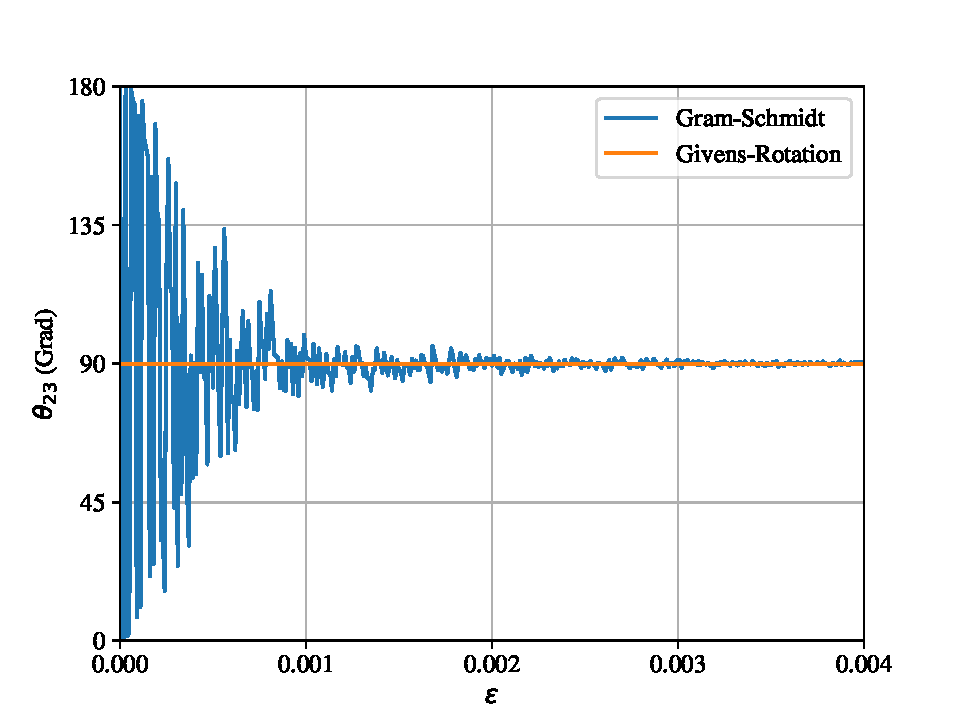
\includegraphics[width=0.9\textwidth]{papers/qr/pics/comp.pdf}
	\caption{Winkel zwischen $q_2$ und $q_3$.\label{qr:comp}}
\end{figure}
Klar ersichtlich ist, wie stabil die Implementation mit den Givens-Rotationen immer einen Winkel von $90^\circ$ liefert, die Implementation mit dem Gram-Schmidt-Orthonormalisierungsverfahren dagegen sehr instabil wirkt.

Die $QR$-Zerlegung über das Gram-Schmidt-Orthonormalisierungsverfahren liefert zwar eine sehr intuitive Methode, ist aber numerisch nicht stabil und sollte deshalb nicht so verwendet werden.
Bessere numerische Eigenschaften bringt eine Implementation mit Givens-Rotationen mit sich.